% Options for packages loaded elsewhere
\PassOptionsToPackage{unicode}{hyperref}
\PassOptionsToPackage{hyphens}{url}
%
\documentclass[
  hyperref,]{ctexart}
\usepackage{lmodern}
\usepackage{amssymb,amsmath}
\usepackage{ifxetex,ifluatex}
\ifnum 0\ifxetex 1\fi\ifluatex 1\fi=0 % if pdftex
  \usepackage[T1]{fontenc}
  \usepackage[utf8]{inputenc}
  \usepackage{textcomp} % provide euro and other symbols
\else % if luatex or xetex
  \usepackage{unicode-math}
  \defaultfontfeatures{Scale=MatchLowercase}
  \defaultfontfeatures[\rmfamily]{Ligatures=TeX,Scale=1}
\fi
% Use upquote if available, for straight quotes in verbatim environments
\IfFileExists{upquote.sty}{\usepackage{upquote}}{}
\IfFileExists{microtype.sty}{% use microtype if available
  \usepackage[]{microtype}
  \UseMicrotypeSet[protrusion]{basicmath} % disable protrusion for tt fonts
}{}
\makeatletter
\@ifundefined{KOMAClassName}{% if non-KOMA class
  \IfFileExists{parskip.sty}{%
    \usepackage{parskip}
  }{% else
    \setlength{\parindent}{0pt}
    \setlength{\parskip}{6pt plus 2pt minus 1pt}}
}{% if KOMA class
  \KOMAoptions{parskip=half}}
\makeatother
\usepackage{xcolor}
\IfFileExists{xurl.sty}{\usepackage{xurl}}{} % add URL line breaks if available
\IfFileExists{bookmark.sty}{\usepackage{bookmark}}{\usepackage{hyperref}}
\hypersetup{
  hidelinks,
  pdfcreator={LaTeX via pandoc}}
\urlstyle{same} % disable monospaced font for URLs
\usepackage[margin=1in]{geometry}
\setlength{\emergencystretch}{3em} % prevent overfull lines
\providecommand{\tightlist}{%
  \setlength{\itemsep}{0pt}\setlength{\parskip}{0pt}}
\setcounter{secnumdepth}{5}
\usepackage{graphicx}
\usepackage{float}
\usepackage{indentfirst}
\setlength{\parindent}{4em}

\author{}
\date{}

\setCJKmainfont[BoldFont=SimHei,ItalicFont=STKaiti]{SimSun}

\begin{document}
\begin{titlepage}

\newcommand{\HRule}{\rule{\linewidth}{0.5mm}} % Defines a new command for the horizontal lines, change thickness here

\center % Center everything on the page
 
%----------------------------------------------------------------------------------------
%	HEADING SECTIONS
%----------------------------------------------------------------------------------------

\textsc{\LARGE Central University of Finance and Economics}\\[1.5cm] % Name of your university/college

\includegraphics[scale=1]{cufe.jpg}\\[1cm] % Include a department/university logo - this will require the graphicx package
\textsc{\Large 中央财经大学}\\[0.5cm] % Major heading such as course name
\textsc{\Large 数学与统计建模案例}\\[0.5cm] % Minor heading such as course title

%----------------------------------------------------------------------------------------
%	TITLE SECTION
%----------------------------------------------------------------------------------------

\HRule \\[0.4cm]
{ \huge \bfseries 29组}\\[0.4cm] % Title of your document
\HRule \\[1.5cm]
 
%----------------------------------------------------------------------------------------
%	AUTHOR SECTION
%----------------------------------------------------------------------------------------

\begin{minipage}{0.4\textwidth}
\textsc{\large }\\[0.5cm] % Minor heading such as course title
\textsc{\large wuyuchong.com}\\[0.5cm] % Minor heading such as course title
\textsc{\large 指导老师:杨欣欣}\\[0.5cm] % Minor heading such as course title
\textsc{\large 统计与数学学院}\\[0.5cm] % Minor heading such as course title
\end{center}

\end{minipage}\\[2cm]

% If you don't want a supervisor, uncomment the two lines below and remove the section above
%\Large \emph{Author:}\\
%John \textsc{Smith}\\[3cm] % Your name

%----------------------------------------------------------------------------------------
%	DATE SECTION
%----------------------------------------------------------------------------------------

{\large \today}\\[2cm] % Date, change the \today to a set date if you want to be precise

\vfill % Fill the rest of the page with whitespace

\end{titlepage}
{
\setcounter{tocdepth}{2}
\tableofcontents
}
\newpage

\hypertarget{ara}{%
\section{ARA}\label{ara}}

\begin{figure}[H]

{\centering \includegraphics[width=0.8\linewidth]{第一次作业_files/figure-latex/unnamed-chunk-3-1} 

}

\caption{ARA指标分布密度图(红色代表ST)}\label{fig:unnamed-chunk-3}
\end{figure}

由图可知,当ARA值较小时,上市公司的财务数据出现异常的概率低于数据正常的概率;随着ARA值逐渐增加,上市公司的财务数据出现异常的概率和数据正常的概率均呈下降趋势,但数据异常的可能性大于数据正常的可能性。

\hypertarget{ux6210ux957fux7387}{%
\section{成长率}\label{ux6210ux957fux7387}}

1999年和2000年,财务数据正常的上市公司销售收入增长率集中在0左右,财务数据出现异常的上市公司销售收入呈现负增长。

\begin{figure}[H]

{\centering 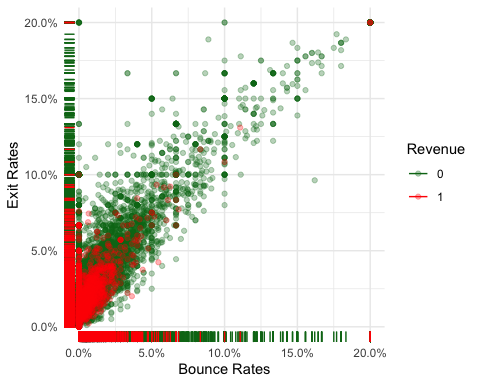
\includegraphics[width=0.8\linewidth]{第一次作业_files/figure-latex/unnamed-chunk-4-1} 

}

\caption{成长率各指标箱线图(红色代表ST)}\label{fig:unnamed-chunk-4}
\end{figure}

\hypertarget{ux5404ux6307ux6807}{%
\section{各指标}\label{ux5404ux6307ux6807}}

\begin{figure}[H]

{\centering 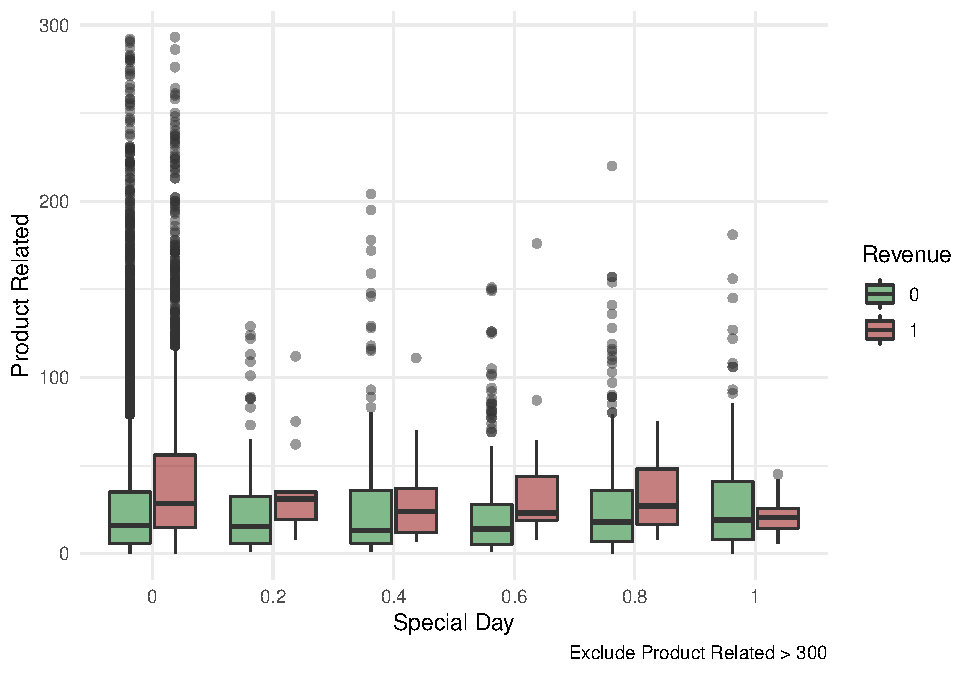
\includegraphics[width=0.8\linewidth]{第一次作业_files/figure-latex/unnamed-chunk-6-1} 

}

\caption{各指标箱线图(红色代表ST)}\label{fig:unnamed-chunk-6}
\end{figure}

对各自变量ST不同情况下绘制箱线图,由图可知,标准化后数据基本服从正态分布,ARA、GROWTH、ROA、SHARE变量在ST不同情况下均值差异较大,说明其取值大小对ST影响较大,其中,ARA为正影响,GROWTH、ROA、SHARE为负影响。

\end{document}